% Inserir antes da seção "Síntese do desempenho nas condições experimentais".
% Requer apenas os pacotes graphicx e float, já usados no capítulo.

\section{Explicabilidade do modelo nos cenários experimentais}
\label{sec:xai_cenarios}

Além da avaliação preditiva, aplicou-se inteligência artificial explicável
(\textit{Explainable Artificial Intelligence} -- XAI) aos três cenários
experimentais. O trabalho de \citet{brar2025xai} empregou Grad-CAM e LIME para
evidenciar as regiões de imagens que sustentaram as decisões de uma rede
neural convolucional. No presente estudo, entretanto, as entradas são variáveis
tabulares, formadas pelas respostas dos sensores MQ e por atributos
ambientais, e o classificador que originou as matrizes de confusão é baseado
em árvores. Por essa razão, adotou-se o método SHAP
(\textit{SHapley Additive exPlanations}) com o algoritmo
\textit{TreeExplainer}, preservando o objetivo de tornar explícita a
contribuição das entradas para as decisões do modelo, mas utilizando uma
técnica compatível com a estrutura dos dados e do classificador.

As explicações foram calculadas exclusivamente sobre os conjuntos de teste. Em
cada cenário, utilizou-se uma amostra determinística de até 2.000 leituras,
balanceada por coleta e classe, para evitar que coletas mais longas dominassem
a análise. Foi explicada a saída relativa à classe com nematoide. Assim,
valores SHAP positivos deslocam a saída do modelo em direção à classe com
nematoide, enquanto valores negativos a deslocam em direção à classe sem
nematoide. A importância global de cada variável foi estimada pela média do
valor SHAP absoluto. Também foram produzidas explicações locais para casos
representativos das células não vazias de cada matriz de confusão.

A Figura~\ref{fig:comparacao_shap_cenarios} compara a participação percentual
de cada variável na importância SHAP total de cada cenário. A normalização
percentual facilita a comparação entre modelos e conjuntos com escalas de
valores SHAP distintas.

\begin{figure}[H]
    \centering
    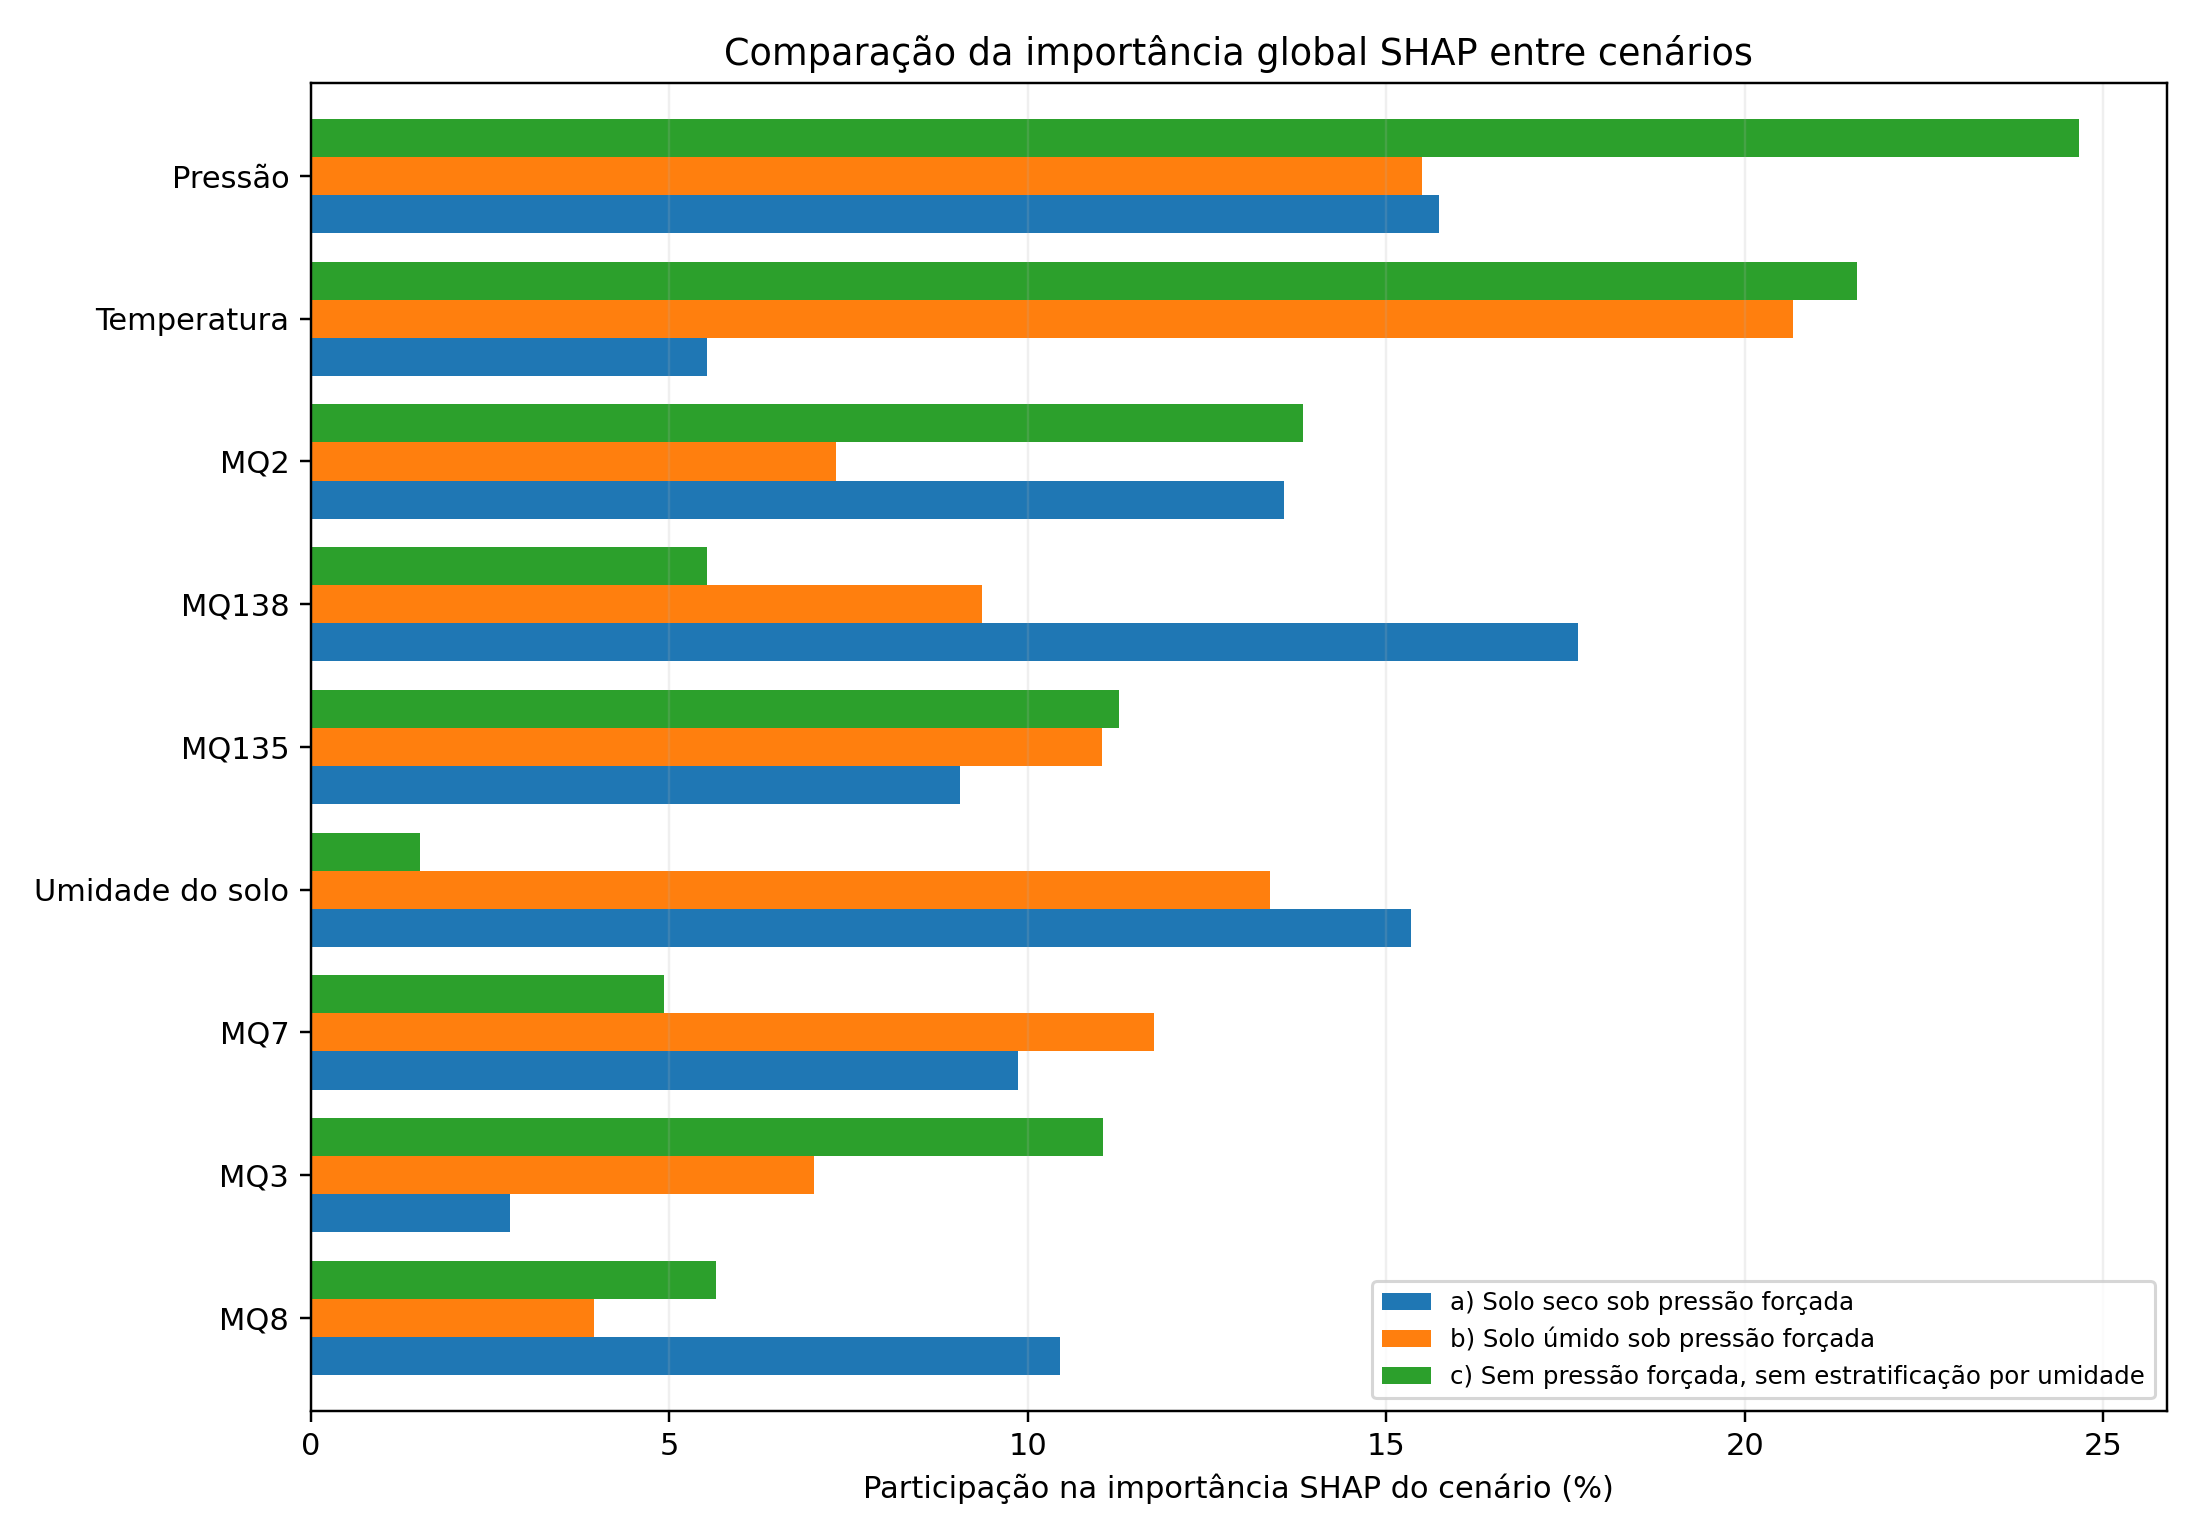
\includegraphics[width=\textwidth]{xai_todos_cenarios/resultados/comparacao_importancia_shap_percentual.png}
    \caption{Comparação da importância global SHAP entre os três cenários experimentais. A importância corresponde à média do valor SHAP absoluto para a classe com nematoide, normalizada para totalizar 100\% em cada cenário.}
    \label{fig:comparacao_shap_cenarios}
    \fonte{Elaborado pelo autor (2026).}
\end{figure}

A Tabela~\ref{tab:top3_shap_cenarios} apresenta as três variáveis mais
influentes em cada condição. No solo seco sob pressão forçada, o sinal
corrigido do MQ-138 foi a variável individual mais importante (17,67\%),
seguido pela pressão interna (15,73\%) e pelo índice de umidade do solo
(15,34\%). Nesse cenário, o conjunto dos seis sensores MQ respondeu por
63,39\% da importância total, enquanto as três variáveis ambientais somaram
36,61\%.

\begin{table}[H]
    \centering
    \caption{Três variáveis de maior importância global SHAP em cada cenário.}
    \label{tab:top3_shap_cenarios}
    \begin{tabular}{p{5.4cm}lcc}
        \hline
        \textbf{Cenário} & \textbf{Posição} & \textbf{Variável} &
        \textbf{Importância (\%)} \\
        \hline
        a) Solo seco sob pressão forçada
        & 1 & MQ-138 corrigido & 17,67 \\
        & 2 & Pressão & 15,73 \\
        & 3 & Umidade do solo & 15,34 \\
        \hline
        b) Solo úmido sob pressão forçada
        & 1 & Temperatura & 20,67 \\
        & 2 & Pressão & 15,50 \\
        & 3 & Umidade do solo & 13,37 \\
        \hline
        c) Sem pressão forçada, sem estratificação por umidade
        & 1 & Pressão & 24,65 \\
        & 2 & Temperatura & 21,56 \\
        & 3 & MQ-2 & 13,84 \\
        \hline
    \end{tabular}
    \fonte{Elaborado pelo autor (2026).}
\end{table}

No solo úmido sob pressão forçada, a temperatura apresentou a maior
contribuição (20,67\%), seguida pela pressão (15,50\%) e pela umidade do solo
(13,37\%). As variáveis ambientais, em conjunto, responderam por 49,54\% da
importância, participação superior à observada no solo seco. Essa mudança é
compatível com a redução de desempenho verificada nessa condição e indica
que as decisões do modelo se tornaram mais dependentes do contexto físico da
aquisição.

No protocolo sem pressão forçada e sem estratificação por umidade, a pressão
registrada foi a variável mais influente (24,65\%), seguida pela temperatura
(21,56\%) e pelo MQ-2 (13,84\%). Pressão e temperatura, isoladamente,
concentraram 46,22\% da importância total; incluindo-se a umidade do solo, as
variáveis ambientais totalizaram 47,74\%. Embora a pressão não tenha sido
forçada nesse protocolo, sua leitura permaneceu disponível como variável de
contexto e foi utilizada pelo classificador.

As Figuras~\ref{fig:shap_seco}, \ref{fig:shap_umido} e
\ref{fig:shap_sem_pressao} mostram, além da magnitude, a direção das
contribuições. Cada ponto representa uma leitura de teste; a posição no eixo
horizontal indica seu efeito sobre a saída relativa à presença do nematoide,
e a cor representa o valor observado da variável.

\begin{figure}[H]
    \centering
    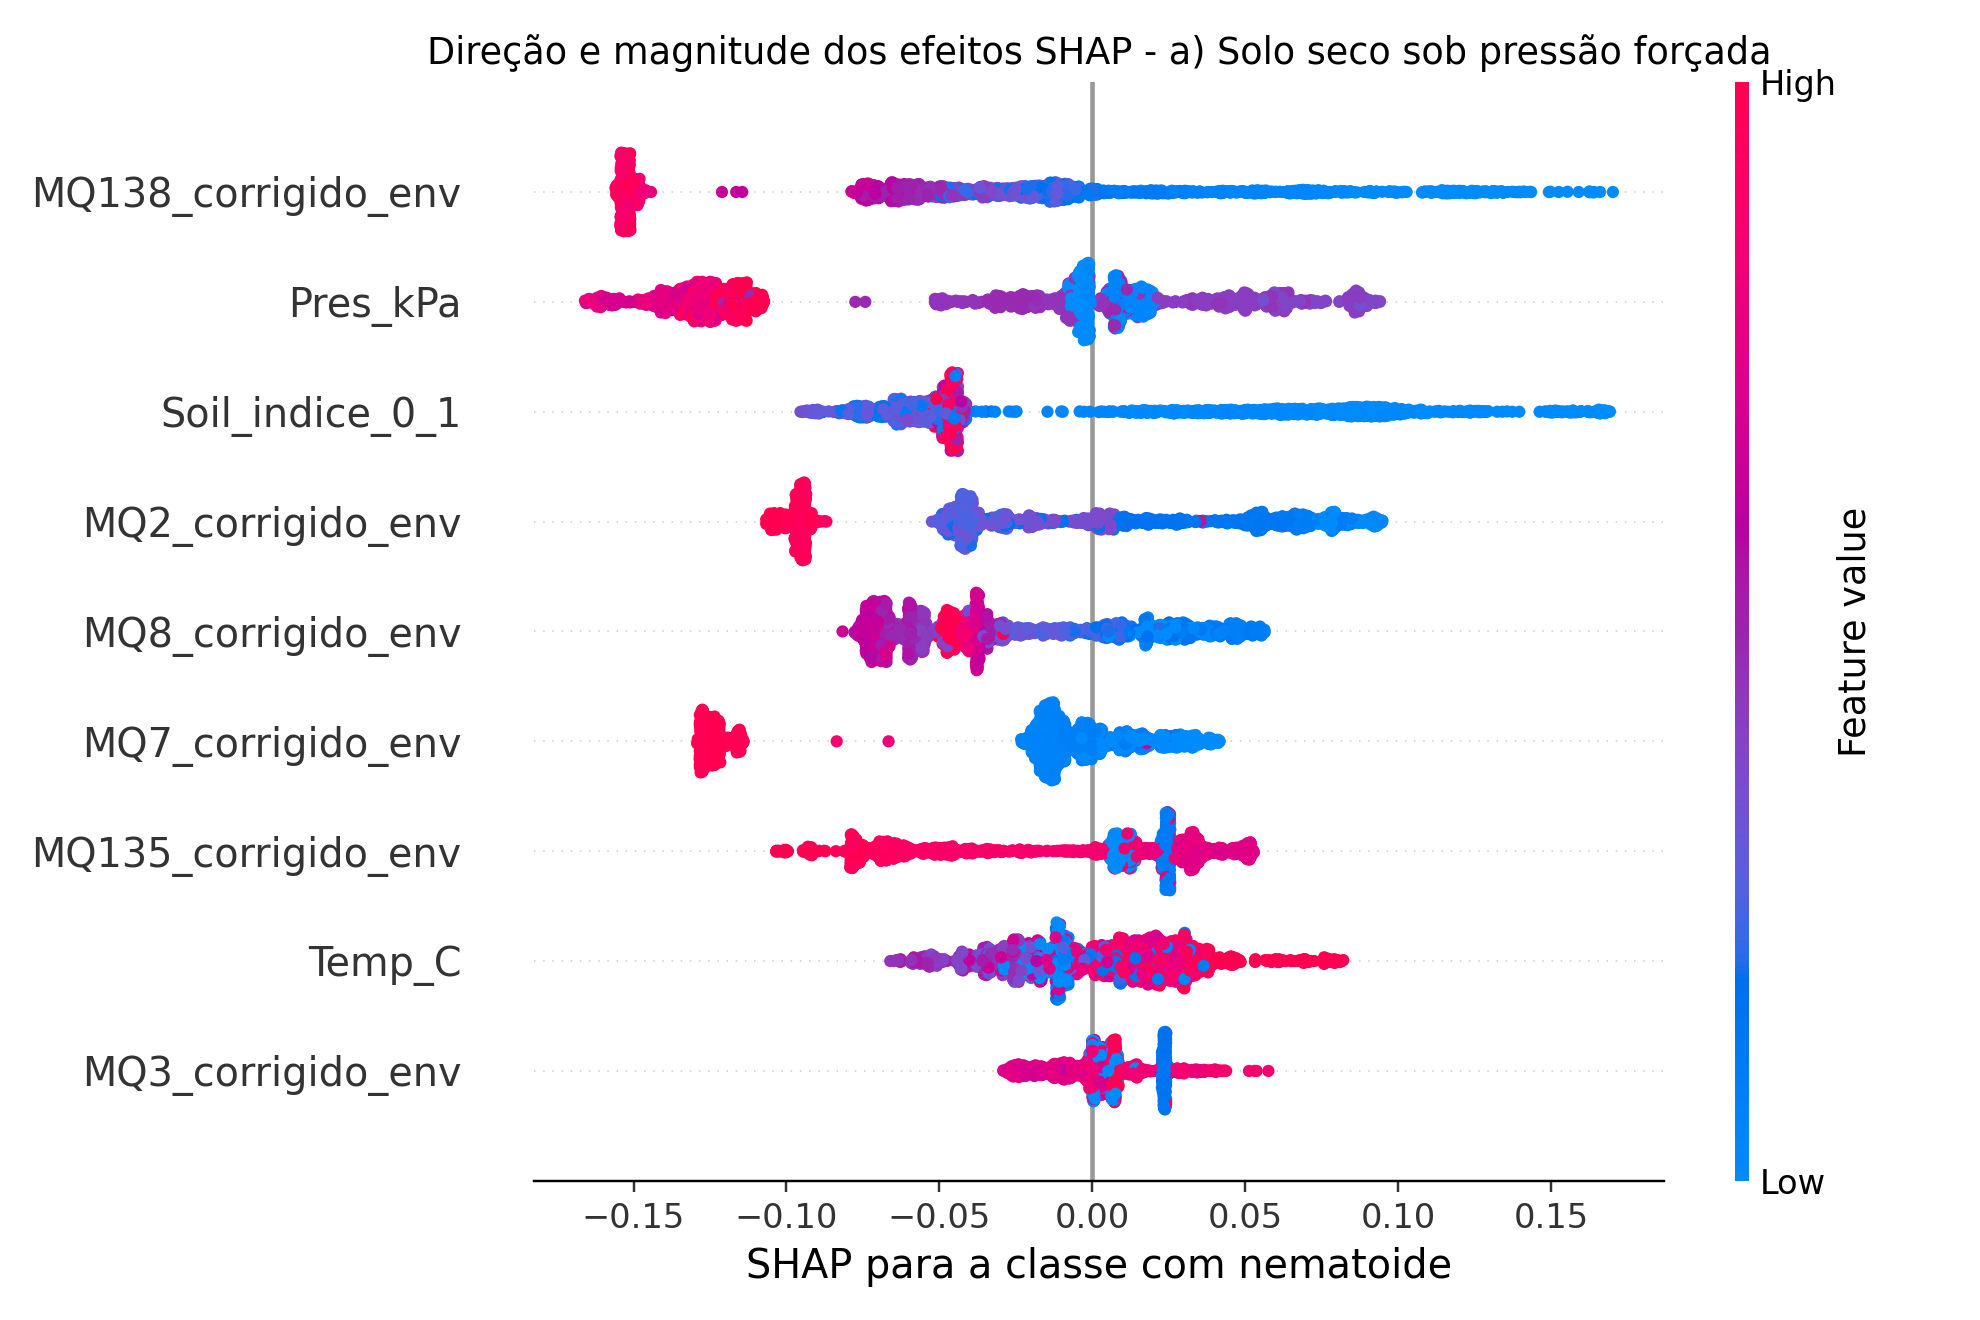
\includegraphics[width=\textwidth]{xai_todos_cenarios/resultados/a_solo_seco_com_pressao/02_resumo_shap_beeswarm.png}
    \caption{Distribuição dos valores SHAP no cenário a) solo seco sob pressão forçada.}
    \label{fig:shap_seco}
    \fonte{Elaborado pelo autor (2026).}
\end{figure}

\begin{figure}[H]
    \centering
    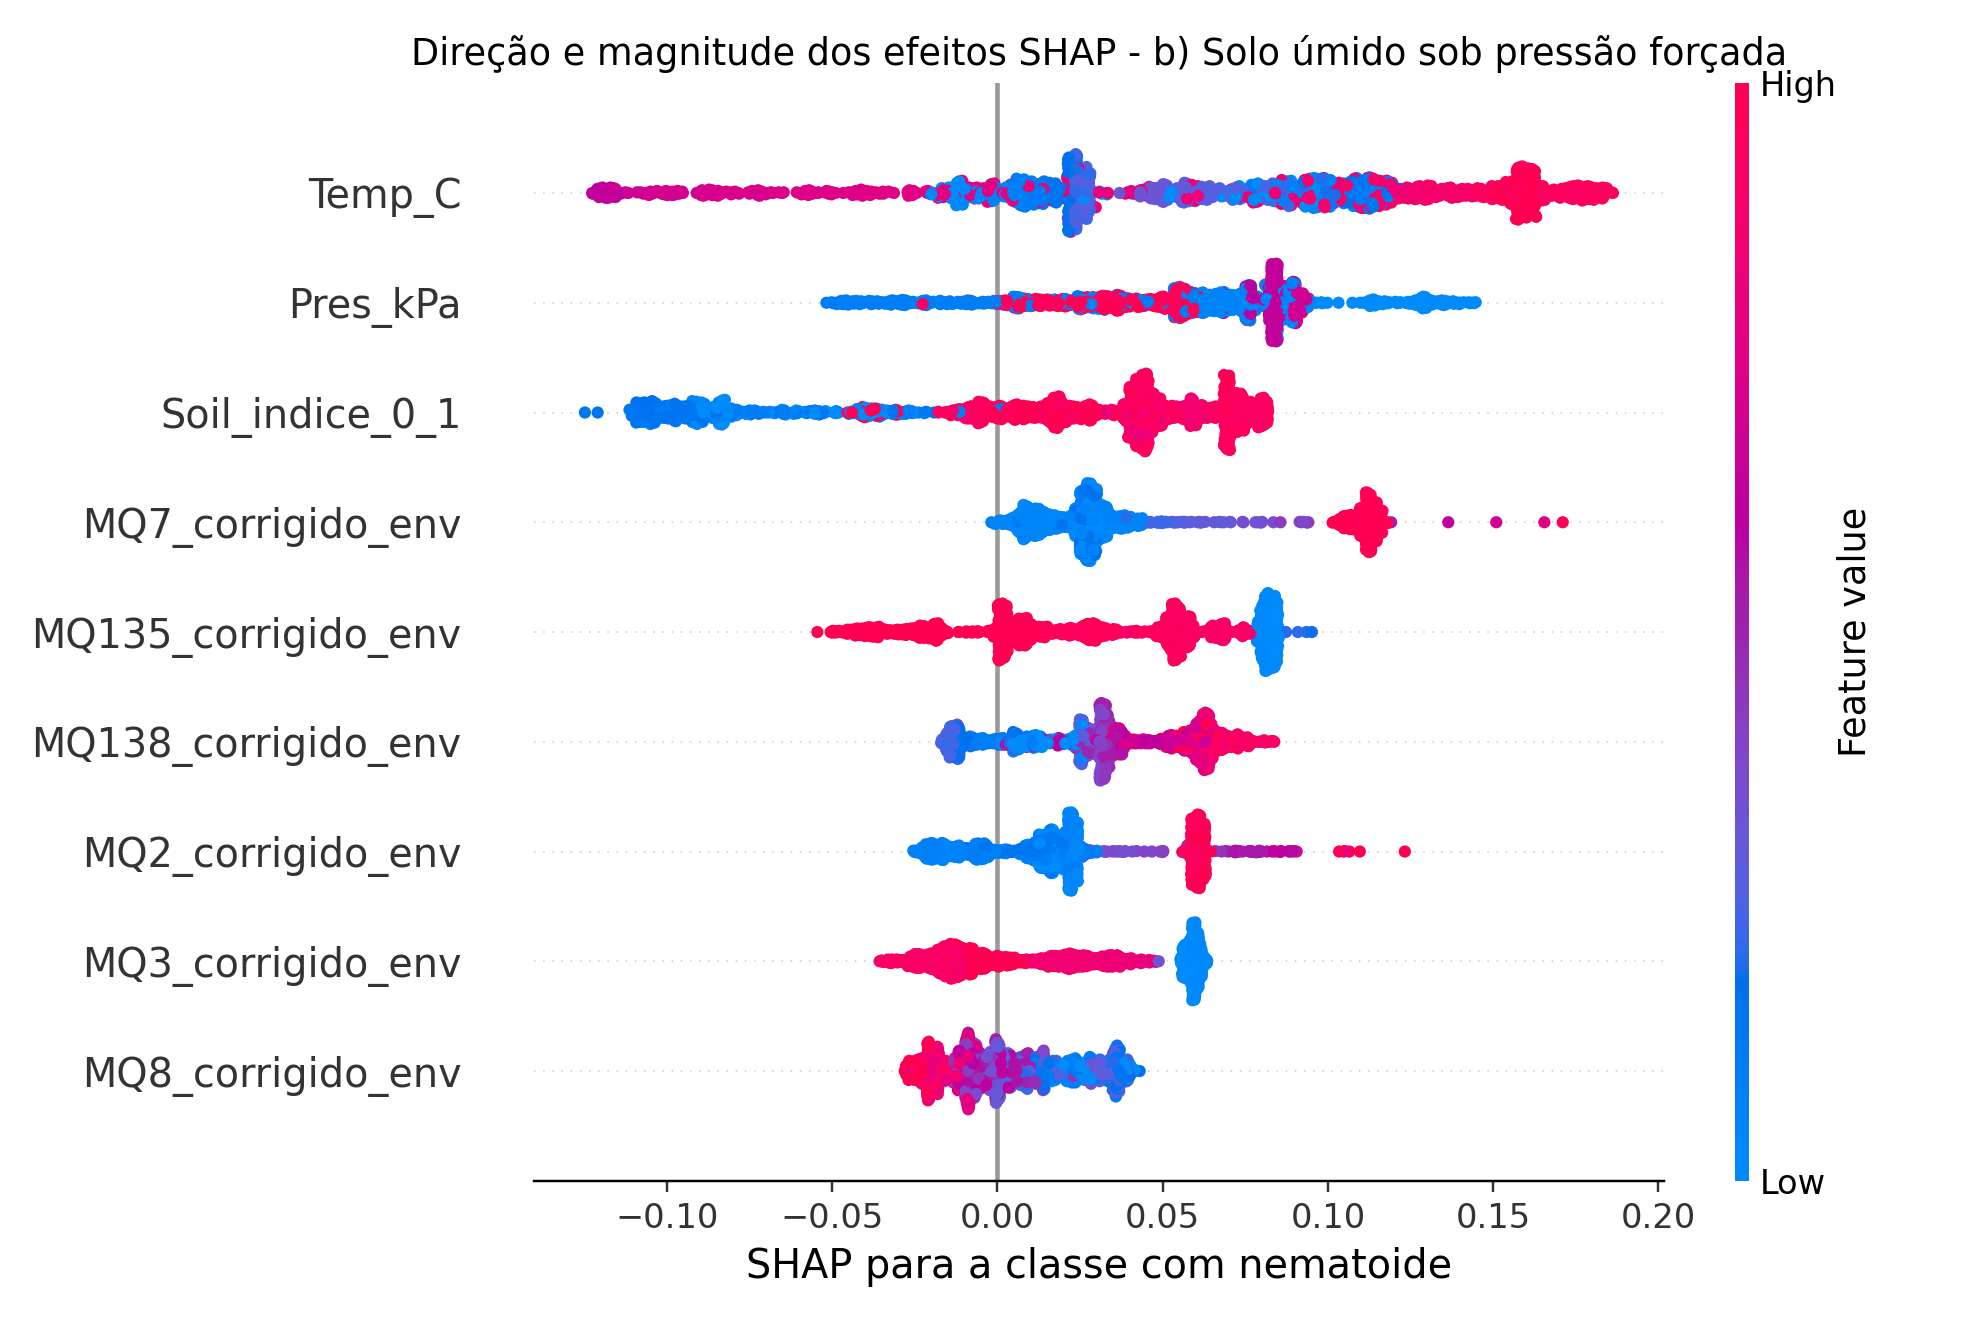
\includegraphics[width=\textwidth]{xai_todos_cenarios/resultados/b_solo_umido_com_pressao/02_resumo_shap_beeswarm.png}
    \caption{Distribuição dos valores SHAP no cenário b) solo úmido sob pressão forçada.}
    \label{fig:shap_umido}
    \fonte{Elaborado pelo autor (2026).}
\end{figure}

\begin{figure}[H]
    \centering
    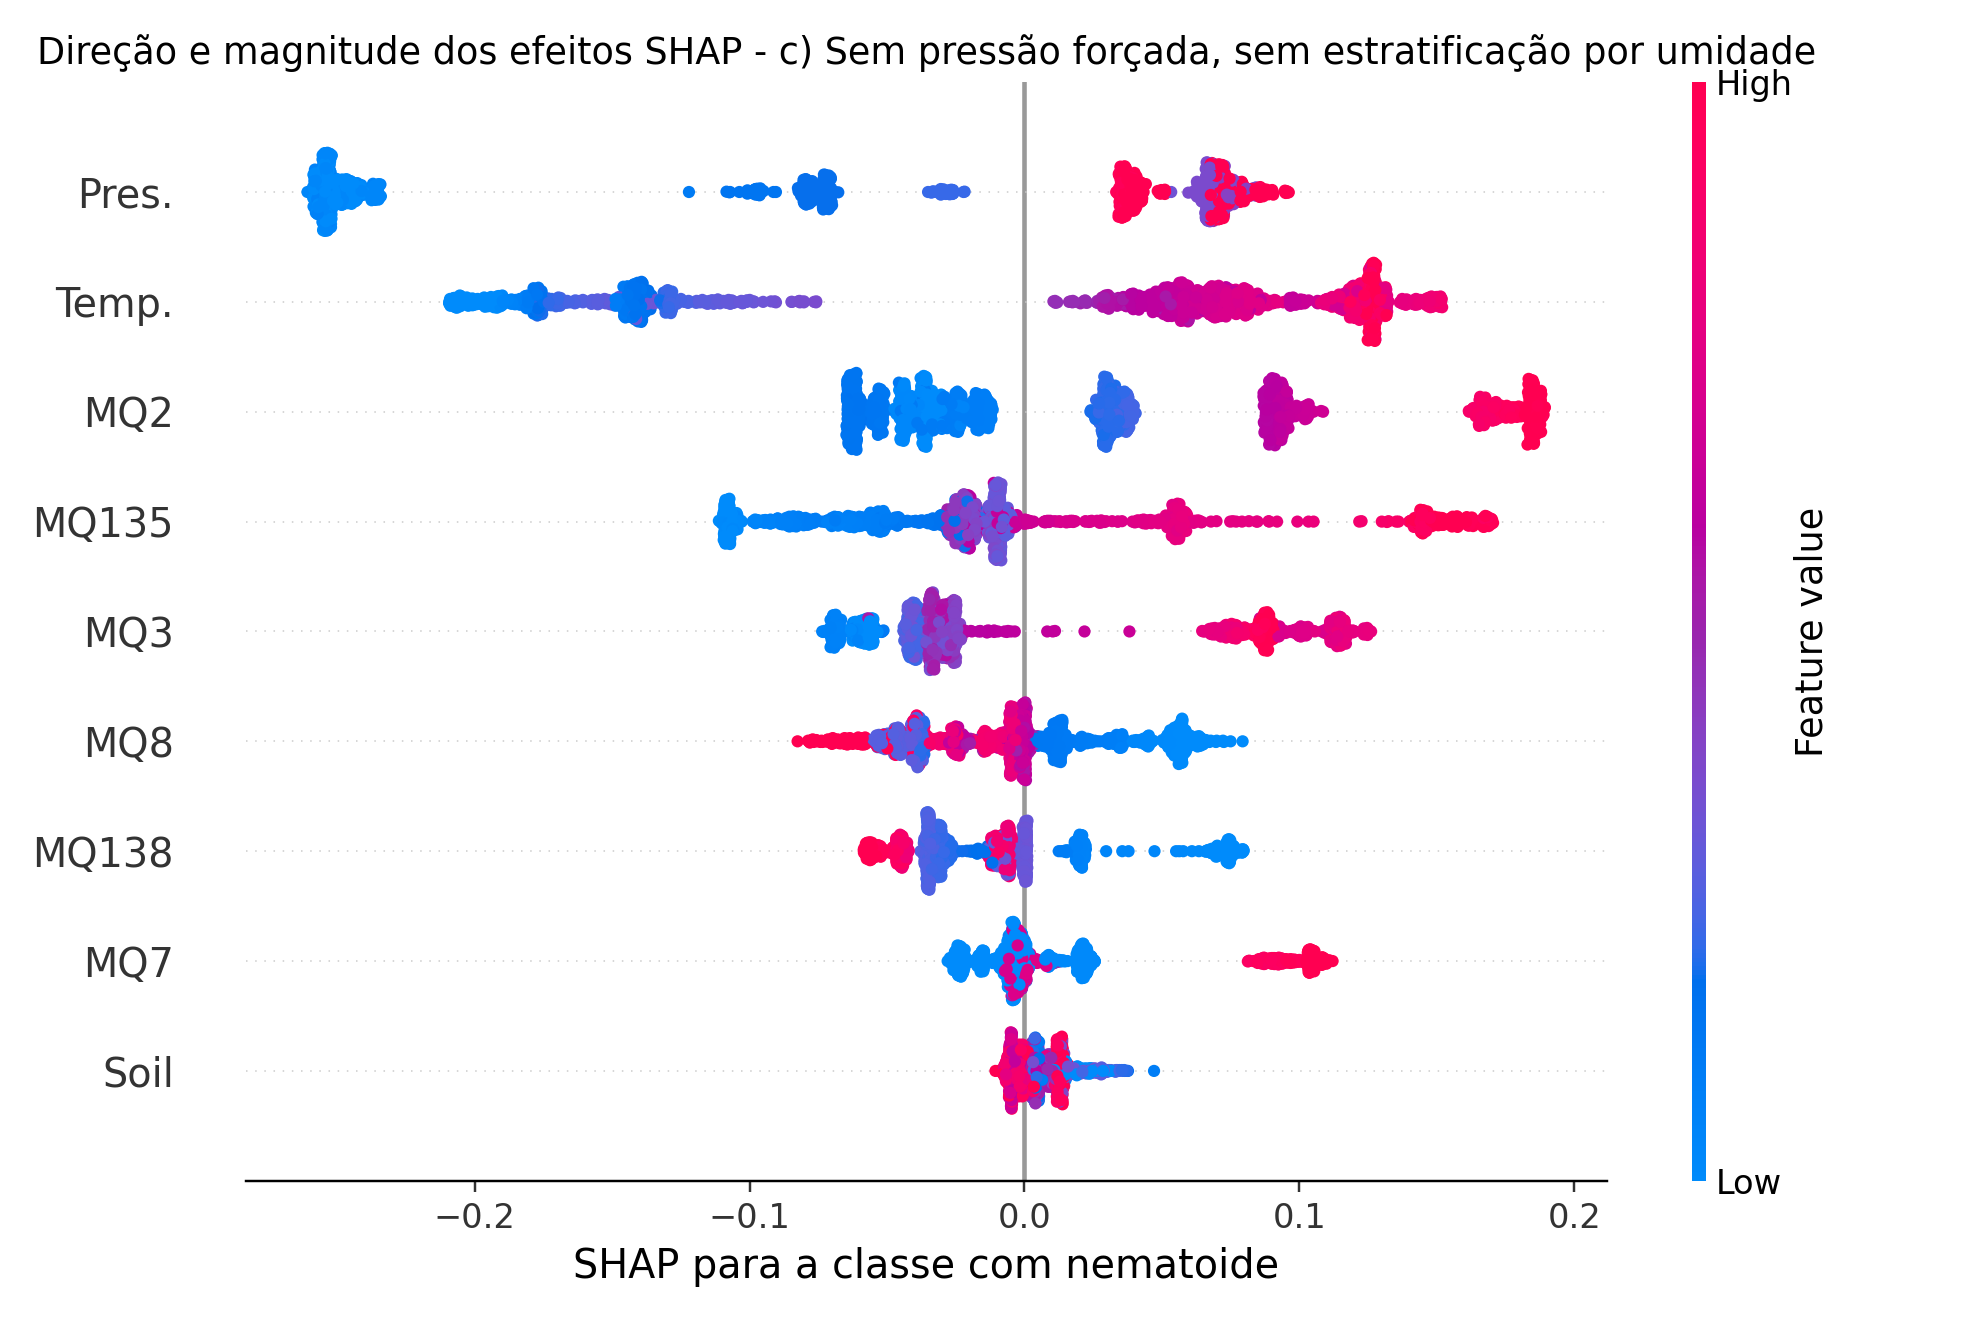
\includegraphics[width=\textwidth]{xai_todos_cenarios/resultados/c_sem_pressao_sem_estratificacao/02_resumo_shap_beeswarm.png}
    \caption{Distribuição dos valores SHAP no cenário c) sem pressão forçada e sem estratificação por umidade.}
    \label{fig:shap_sem_pressao}
    \fonte{Elaborado pelo autor (2026).}
\end{figure}

Os resultados de XAI não demonstram que uma variável seja causa biológica da
presença do nematoide. Eles descrevem as associações utilizadas pelo
classificador para produzir suas previsões. A elevada contribuição da
pressão, da temperatura e da umidade do solo, sobretudo nos cenários b e c,
reforça a necessidade de controlar essas condições em novos ensaios e de
realizar análises de ablação que comparem modelos com apenas sensores MQ,
apenas variáveis ambientais e ambos os grupos. Essa verificação é necessária
para distinguir uma possível assinatura de compostos orgânicos voláteis de
efeitos do protocolo de aquisição, da câmara, da vedação ou do ambiente.
